\documentclass[xcolor=table]{beamer}

\usetheme[secheader,compress]{Madrid} %Primary theme

\usepackage{verbatim}
\usepackage{graphicx}

%% UTM Colors
\definecolor{UTMblue}{rgb}{0.043137, 0.137254, 0.254901}
\definecolor{UTMorange}{rgb}{1.0, 0.509803, 0}

\setbeamercolor{palette primary}{bg=UTMblue,fg=white}
\setbeamercolor{palette secondary}{bg=UTMblue,fg=white}
\setbeamercolor{palette tertiary}{bg=UTMblue,fg=white}
\setbeamercolor{palette quaternary}{bg=UTMblue,fg=white}
\setbeamercolor{structure}{fg=UTMblue} % itemize, enumerate, etc
\setbeamercolor{section in toc}{fg=UTMblue} % TOC sections
\setbeamercolor{title}{fg=UTMorange}

\setbeamercolor{subsection in head/foot}{bg=UTMorange,fg=white}

%%%%%%%%%%% BEGIN MACROS %%%%%%%%%%%%%%%%%%
% frameT: Frame with title
\newcommand{\frameT}[2]{\frame{\frametitle{#1} #2}}

% frameF: Fragile frame with title
\newcommand{\frameF}[2]{
  \begin{frame}[fragile]
    \frametitle{#1}
    #2
  \end{frame}
}

% frameTop: Frame aligned t the top
\newcommand{\frameTop}[2]{\frame[t]{\frametitle{#1} #2}}


\newcommand{\tab}{\hspace{1cm}}

\newcommand{\spaceor}{\hspace{5pt} \textbf{or} \hspace{5pt}}

%%%%%%%%%%% END MACROS %%%%%%%%%%%%%%%%%%%%



\begin{document}

\title{The Deep Journey}

\author{James Blankenship and Andrew Marshall}
\institute{UT-Martin}
\date{\today}

%%%%%%%%%%% BEGIN TITLE %%%%%%%%%%%%%%%%%%
\frame{\titlepage}

 %\section{Outline}
%%%%%%%%%%%% END TITLE  %%%%%%%%%%%%%%%%%%



\section{Introduction}

  
  \section{Background}
  \frameT{Overview}{
    
  Overview of project 
  \bigskip
  \begin{enumerate}

  \item Real time combat game in Unreal Engine
    \bigskip
    \item It will be in the first person where it will be viewed from the players eyes
    \bigskip
  \item Multiple levels in game and it will be in the fantasy genre.
   
  \end{enumerate}
  }
  \frameT{Overview}{
  \section{Overview cont.}
  
  Overview of Project cont.
  \begin{enumerate}
    \item Each level will focus on a enemy race.
    \bigskip
  \item Enemy types are orcs, goblins, and humans.
    \bigskip
  \item There will be weapon upgrades such as increased damage.
    \bigskip
    \item Character will have access to magic, and other abilites 
       \bigskip
    \item Magic such as pyromancy,faith magic,and sorcery.
  \end{enumerate}
  }
  


 


  \frameT{Project Goals} {
    \begin{enumerate}
  \item There are 3 different levels.
    \bigskip
  \item The three levels are  the castle level,castle basement, and the woods area.
    \bigskip
  \item The  player character will have  different classes. 
  
    \bigskip
  \item Program different AI enemies.\\
  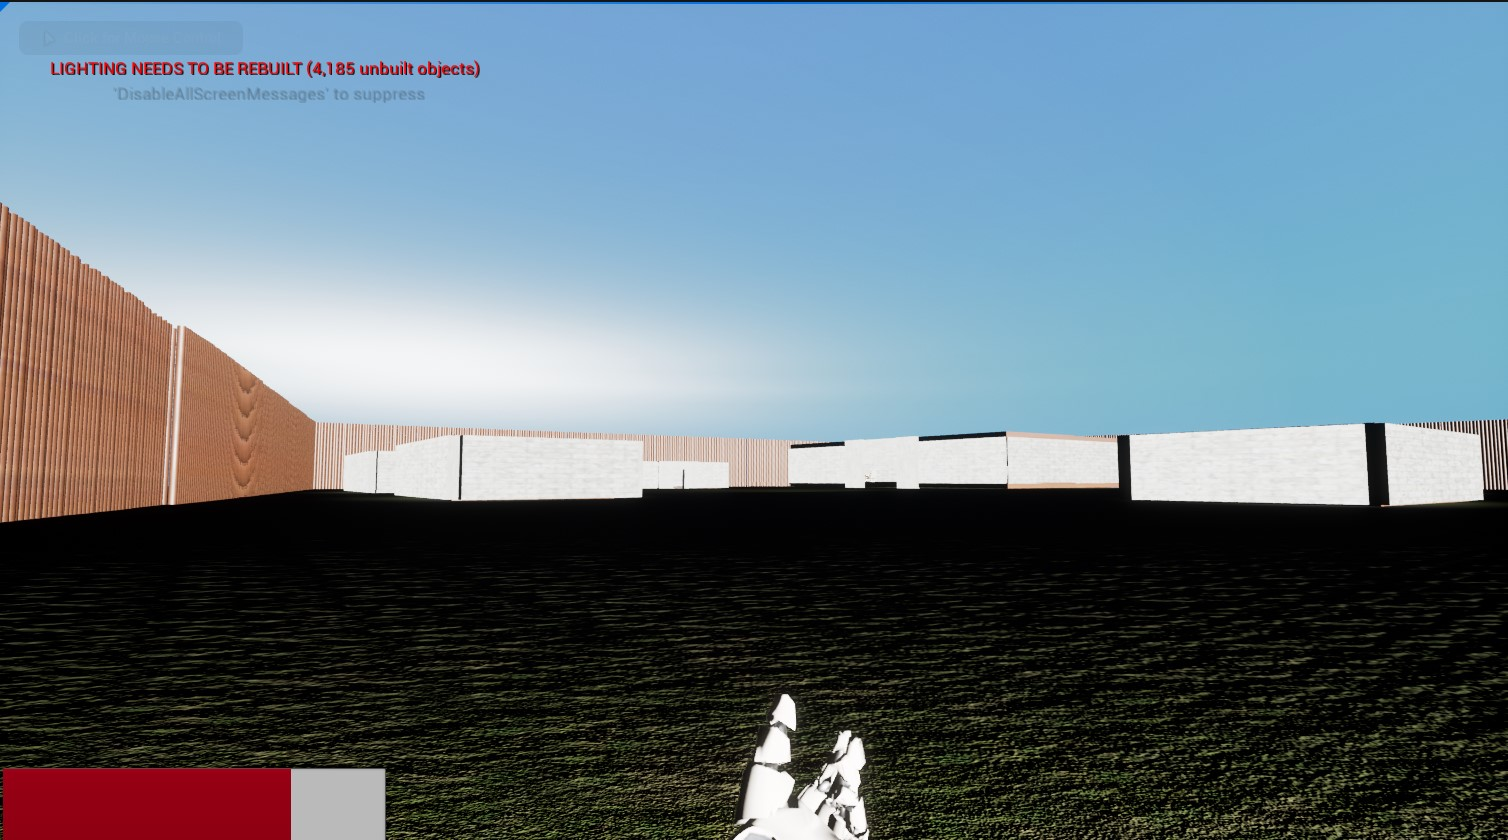
\includegraphics[width=4cm, height=4cm]{figures/woods.jpg}
  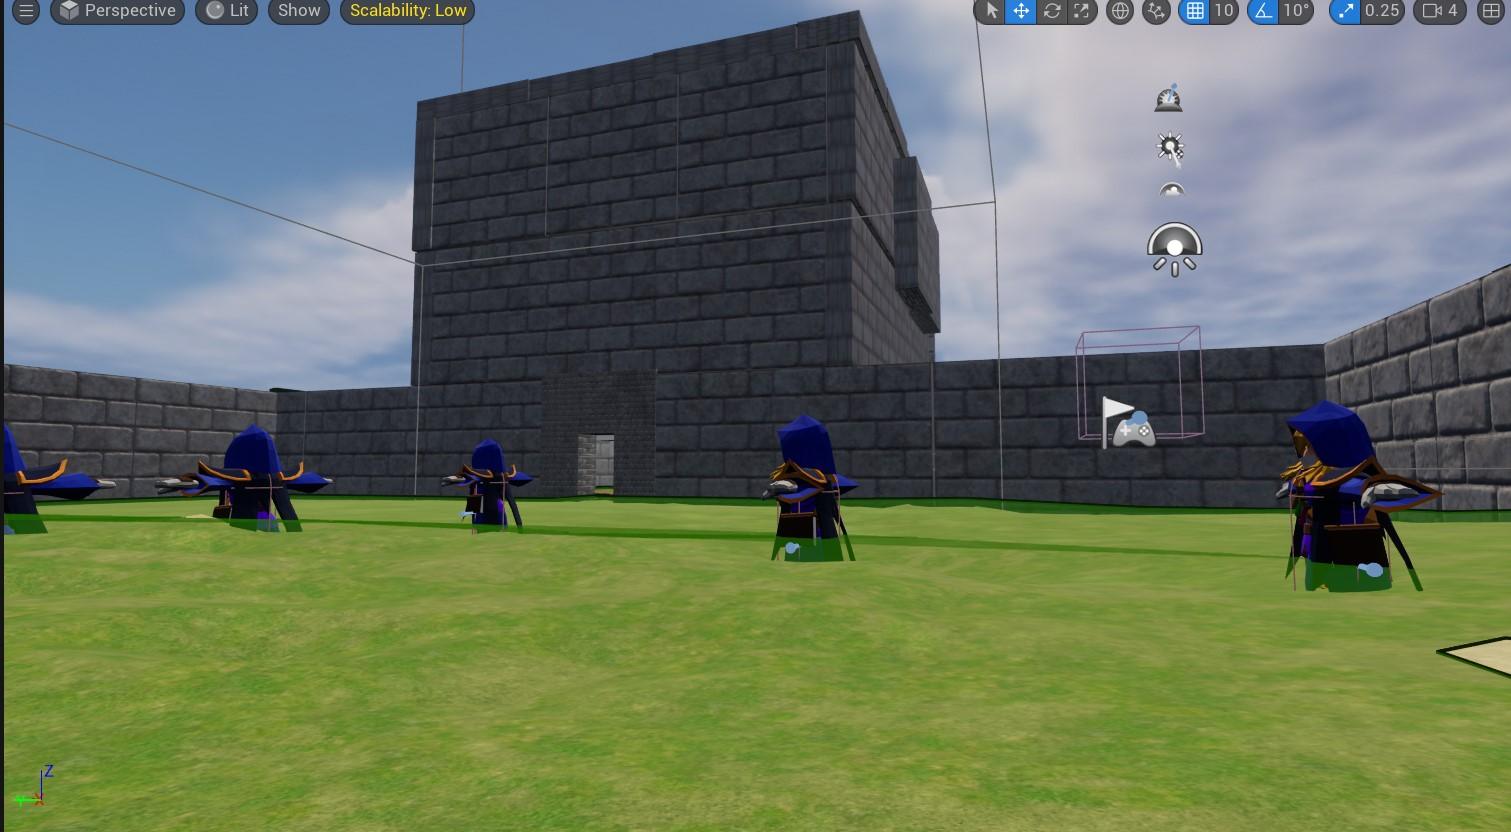
\includegraphics[width=4cm, height=4cm]{figures/castle.jpg}
  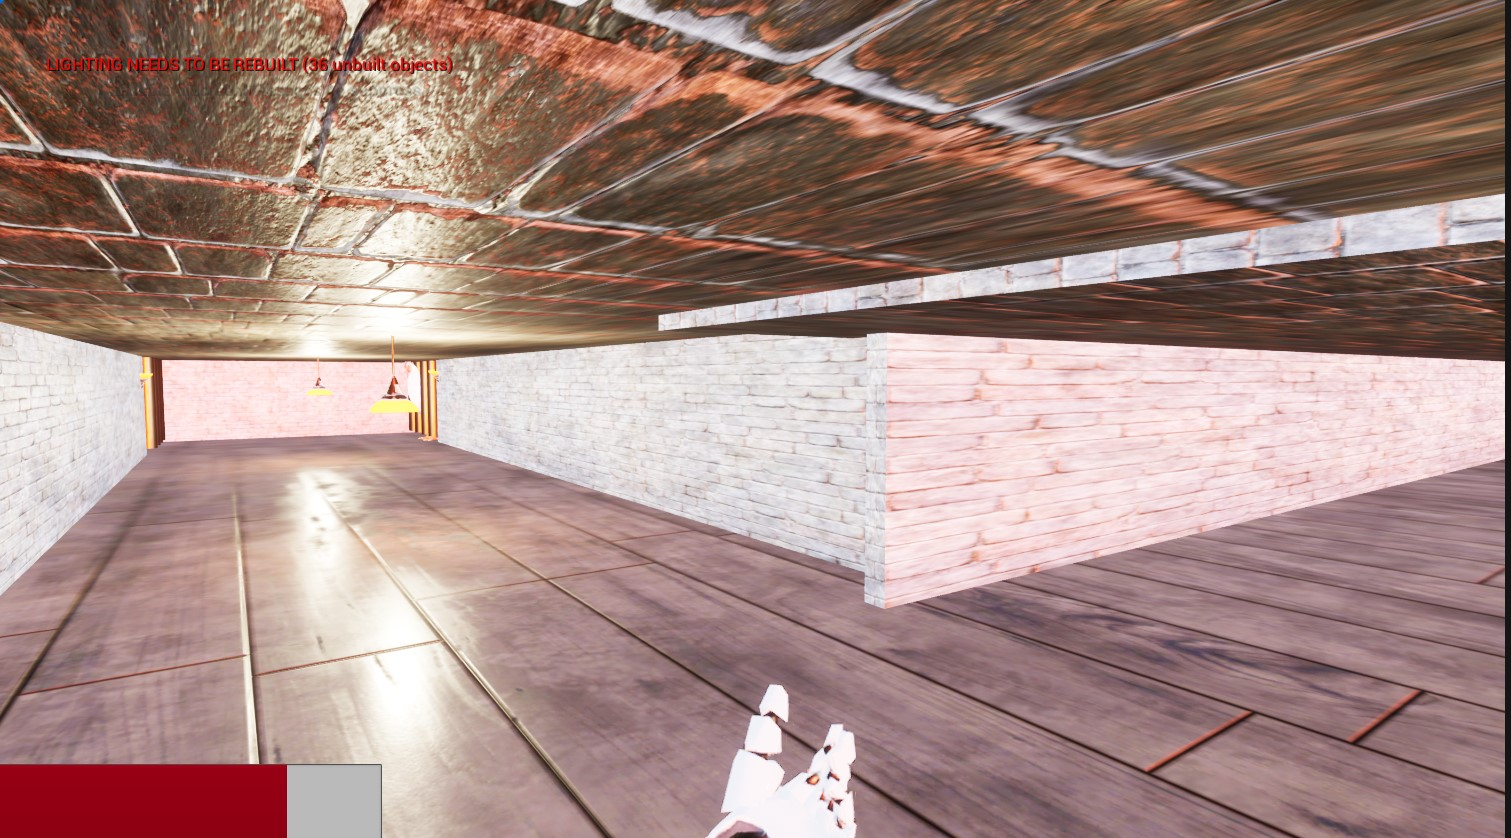
\includegraphics[width=3cm, height=4cm]{figures/basement.jpg}
    \end{enumerate}
}

\begin{frame}[fragile]
\frametitle{Technology used}

\begin{enumerate}
    \item The game was developed using unreal engine 5.
    \bigskip
  \item To help with collabaration and version control we used github.
    \bigskip
  \item This presentation was made using latex. 
    \bigskip
    
  \end{enumerate}
\end{frame}

\frameT{Demo slide} {
  \begin{center}
    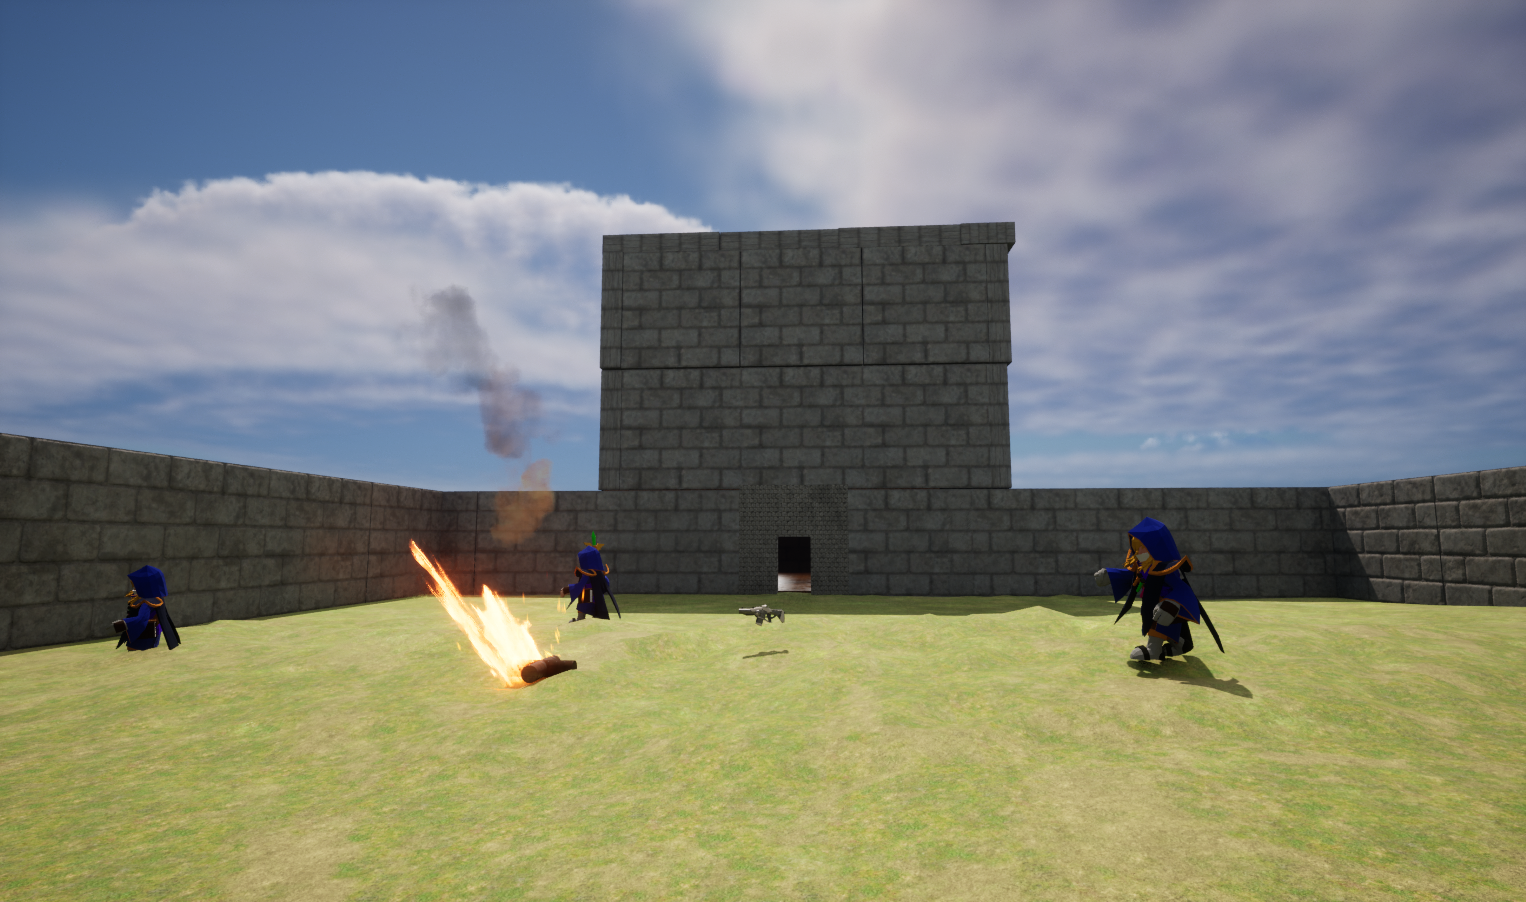
\includegraphics[width=10cm]{figures/unknown.png}
  \end{center}
}


\section{Sections--a useful organizational tool.}



\frameT{Summary}{
  \begin{enumerate}
    \item Any Questions or comments?
    \bigskip
    \item Below is our contact info
    \bigskip
    \item jesamars@ut.utm.edu or jamcblan@ut.utm.edu
    \bigskip
    \item https://github.com/James-Blankenship4276/CSCI-Senior-Project
    \end{enumerate}
}










\frameT{Results} {
  Describe any results of your work here.

  \bigskip

  So far we've created the first two levels and some basic AI.

  \bigskip

  Things that didn't work?
}




%\frameF{fragile test} {
%}

%% \frameF{Prolog Family Tree} {
%% \begin{verbatim}
%% hello
%% \end{verbatim}



%% }

%Empty Page
%\frameT{Frame 1}{
%}  


\end{document}
